%%%%%%%%%%%%%%%%%%%%%%%%%%%%%%%
% COM3502-4502-6502 Speech Processing
% Programming Assignment Response Sheet
% Prof. Roger K. Moore
% University of Sheffield
% 24 October 2020
%%%%%%%%%%%%%%%%%%%%%%%%%%%%%%%

\documentclass[hidelinks,a4paper,11pt]{article}

\usepackage[margin=1.2in]{geometry}
\usepackage{graphicx}
\usepackage{hyperref}
\usepackage[parfill]{parskip}
\usepackage{mdframed}
\usepackage{enumitem,amssymb}
\usepackage{float}
\newcounter{question}
\newcommand\myq{\refstepcounter{question}\thequestion}
\usepackage{gensymb}
\usepackage{tipa}  % IPA symbols
\usepackage[bottom]{footmisc}
\usepackage[UKenglish]{isodate} % Formats the \today command to D-M-Y


\begin{document}

\begin{titlepage}

\begin{center}
{\LARGE University of Sheffield}\\[1cm]
\huge {\bfseries COM3502-4502-6502\\Speech Processing}\\[1cm]
\includegraphics[width=5cm]{tuoslogo.png}\\[1cm]
{\huge \bfseries Programming Assignment}\\[0.5cm]

%vvvvvvvvvvvvvvvvvvvvvvvvvvvvvvvvvvvvvvvvvvvvvvvvvvvvvvvvvvvvvv
% EDIT YOUR NAME
{\Large Boxuan Shan}\\[1cm]
%^^^^^^^^^^^^^^^^^^^^^^^^^^^^^^^^^^^^^^^^^^^^^^^^^^^^^^^^^^^^^^^^^^

{\LARGE Department of Computer Science}\\
{\Large \today}
\end{center}

\end{titlepage}

{\color{red}{\bfseries QUESTION 0}\\What programming environment did you use to develop your code (e.g.\ \texttt{pd-vanilla} or \texttt{pd-extended} on a Mac/Windows/Lunix system)?}
\\
\begin{mdframed}
  pd-vanilla on a Windows 10 system, with externals: ``else'' and ``Gem'' installed.
\end{mdframed}
\vspace*{\baselineskip}

{\color{red}{\bfseries QUESTION \myq\ \emph{(worth up to 5 marks)}}\\Provide a screenshot of \texttt{[wsprobe$\sim$]} for a typical voiced sound, and explain the features in the waveform and spectrum that distinguish it from an unvoiced sound.  \emph{Hint: use the `snapshot' feature in \texttt{[wsprobe$\sim$]} to obtain a static display.}}
\\
\begin{mdframed}
  Obviously, the waveform is periodic, and two typical formants can be observed in the spectrum, they are F1 and F2, as shown in red text in the figure. Therefore, this is a very typical vowel in speech which is a voiced sound. Unvoiced sound do not have periodic waveform and formants in the spectrum.
\begin{figure}[H]
  \begin{center}
    \frame{\includegraphics[width=0.6\textwidth]{Q1.png}}
  \end{center}
\end{figure}
\end{mdframed}
\vspace*{\baselineskip}

{\color{red}{\bfseries QUESTION \myq\  \emph{(worth up to 5 marks)}}\\Which sounds are most affected when the low-pass cut-off frequency is set to around 500 Hz - vowels or consonants - and why?}
\\
\begin{mdframed}
  When the low-pass cut-off frequency is set to about 500Hz, the attenuation effect of consonants is most obvious. Consonants contain a lot of fricatives, and the main energy of fricatives is concentrated on relatively high frequencies, especially for voiceless fricatives. Therefore, when the low-pass cut-off is applied, frequencies above 500 Hz will be greatly attenuated, thereby greatly attenuating the energy of consonants. However, since the main energy of vowels is concentrated on relatively low frequencies, usually lower than 500Hz, it is almost unaffected.
\end{mdframed}
\vspace*{\baselineskip}

{\color{red}{\bfseries QUESTION \myq\ \emph{(worth up to 5 marks)}}\\How is it that the speech is still quite intelligible when the high-pass cut-off frequency is set to 10 kHz?}
\\
\begin{mdframed}
  When the high-pass cut-off frequency is set to 10kHz, the energy of the vowels is greatly attenuated, but the fricatives in the consonants are preserved due to the higher energy frequency. However, in speech, vowels carry less information than consonants, it can be seen as a carrier signal modulated by consonants. Therefore the speech is still quite intelligible when vowels are blurry.
\end{mdframed}
\vspace*{\baselineskip}

{\color{red}{\bfseries QUESTION \myq\ \emph{(worth up to 5 marks)}}\\COM3502-4502-6502: The \texttt{[GraphicEqualiser$\sim$]} object uses an FFT internally; what does FFT stand for and what does an FFT do?\\COM4502-6502 ONLY: What is a DFT and how is it different from an FFT?}
\\
\begin{mdframed}
  The word "FFT" stands for "Fast Fourier Transform", which is an efficient implementation of the Fourier Transform algorithm. It can be used to analysis, in a period of time, the power at different frequencies of a waveform,  which can represent the characteristics of the waveform in the frequency domain. Specifically, the Fourier transform uses Sine and Cosine correlation to calculate the amplitude and phase of a waveform at different frequencies. First, divide the waveform into multiple blocks, apply a window function to each block to prevent leakage, and then calculate the Sine and Cosine correlation at different frequencies for this block of waveform. Through the Sine and Cosine correlation, the amplitude and phase can be obtained.
\end{mdframed}
\vspace*{\baselineskip}

{\color{red}{\bfseries QUESTION \myq\ \emph{(worth up to 10 marks)}}\\With \texttt{speed = 50} and \texttt{depth = 0.5}, what are the minimum and maximum amplitudes of your LFO output, and how do they vary with changes in these two settings?  Also, please provide two screenshots: (a) your \texttt{[LFO$\sim$-help]} object and (b) the internal structure of your \texttt{[LFO$\sim$]} object.}
\\
\begin{mdframed}
  With speed=50 and depth=0.5, the minimum and maximum amplitudes of my LFO output is half of the maximum amplitude range. If the speed is changed, the output amplitude will not change, but the frequency will change. If the depth is changed, the amplitude of the output will change, but the frequency will not change.
\begin{figure}[H]
  \begin{center}
    \frame{\includegraphics[width=0.6\textwidth]{Q5a.png}}
  \end{center}
\end{figure}
\begin{figure}[H]
  \begin{center}
    \frame{\includegraphics[width=0.6\textwidth]{Q5b.png}}
  \end{center}
\end{figure}
\end{mdframed}
\vspace*{\baselineskip}

{\color{red}{\bfseries QUESTION \myq\ \emph{(worth up to 5 marks)}}\\In your own words\footnote{I.e.\ do not plagiarise from Wikipedia.}, why is this effect known as `ring modulation'?}
\\
\begin{mdframed}
  The essence of ring modulation is to use a simple periodic waveform, such as a sine wave, to modulate the payload waveform by multiplying with the payload. This function can be realized by a simple circuit in the early days, which contains a ring structure composed of diodes, thus it is called ring modulation.
\end{mdframed}
\vspace*{\baselineskip}

{\color{red}{\bfseries QUESTION \myq\ \emph{(worth up to 5 marks)}}\\Why is SSB commonly used in long-distance radio voice communications?}
\\
\begin{mdframed}
  After the payload waveform is processed by ring modulation, two symmetrical upper and lower sidebands will be generated, which means that the payload exists in both sidebands at the same time. Therefore, in the transmission process, only one of the sidebands needs to be transmitted to decode the payload, which is called single-sideband modulation (SSB). This method can reduce the energy wasted on the carrier, which is conducive to saving energy and increasing the transmission distance, so it is often used for long-distance transmission.
\end{mdframed}
\vspace*{\baselineskip}

{\color{red}{\bfseries QUESTION \myq\ (\emph{worth up to 5 marks)}}\\COM3502-4502-6502: Why can the voice be shifted up in frequency much further than it can be shifted down in frequency before it becomes severely distorted?  \emph{Hint: look at \texttt{[wsprobe$\sim$]}.}\\COM4502-6502 ONLY: Your frequency shifter changes all the frequencies present in an input signal. How might it be possible to change the pitch of a voice \emph{without} altering the formant frequencies?}
\\
\begin{mdframed}
  Because the main formants of speech are concentrated on lower frequencies, there is a lot of room for upward shifting, while the space for downward shifting is very small. If the downward shifting is excessive, it may produce the artifacts of the mirror image of the main formant, and cause aliasing, thereby causing distortion.
\end{mdframed}
\vspace*{\baselineskip}

{\color{red}{\bfseries QUESTION \myq\ \emph{(worth up to 5 marks)}}\\In a practical system, why is it important to keep the feedback gain less than 1?}
\\
\begin{mdframed}
  From a physical point of view, sound waves propagate and reflect in space to form reverberation, and sound waves will attenuate with distance and time during propagation. Therefore, the intensity of the returned sound waves should be less than the intensity of the sound waves generated by the sound source. In the simulation, the feedback gain should be less than 1 to simulate the attenuation of sound waves. If the feedback gain is equal to or greater than 1, the feedback sound will not decay or it will increase with time, and they will overlap indefinitely. From another point of view, since the filter uses feedback, it is an IFR filter. If the gain of the feedback exceeds 1, this implies a pole in the Z-Plane outside the range of the unit circle, which will cause the filter to become unstable.
\end{mdframed}
\vspace*{\baselineskip}

{\color{red}{\bfseries QUESTION \myq\ \emph{(worth up to 50 marks\footnote{25 for functionality, 15 for design/layout, 5 for \texttt{Pd} features, 5 for innovations})}}\\Please provide a short\footnote{no more than 500 words} description of the operation of your \texttt{[VoiceChanger]} application, together with a screenshot of your final GUI.}
\\
\begin{mdframed}
  Please load the file “[VoiceChanger].pd” to launch the application.

  After launching the application, the input-related configuration panel will be displayed in the upper left corner of the screen, including a file loader and a signal source selector. The upper right corner of the screen will display the configuration panel related to audio output, where you can adjust the output volume and switch the DAC state.

  Below the input panel, a vertical effect chain will be shown, which includes 10 effects. There are switches on the upper right corner of each effect to control the enable or disable of it, where green implies enabled and red implies disabled. In addition, there are mixer panels next to the bottom left corner of each effector, which is used to adjust the wet/dry mixing ratio. Drag the slider to the far left to be pure dry sound, that is, the sound without effects. Drag the slider to the far right to make pure wet sounds, that is, sounds with completely added effects. If it is somewhere in the middle, the dry and wet sounds will be mixed in a certain proportion.

  In each effect, you will see multiple yellow sliders and blue buttons. The yellow sliders represent the basic parameters of the effect. Adjusting them can directly change the output of the effect. The blue buttons represent presets. Click the button to load the preset basic parameters, thereby changing the output of the effect.

  After starting the application, all the effects are enabled by default, and all mixers are adjusted to pure wet sound. It is recommended to turn off all or part of the effects as needed. Then please enable the output at the upper right corner of the screen and adjust the volume to a suitable level. After that, select the desired input type in the signal source selector. If the input type is a file, you need to click ``Open File'' or ``Play'' in the file loader to select an input file. Then you will expect to hear processed audio from your audio output device.

  Each effect can achieve different result:

  \begin{enumerate}
    \item Low-cut: Can be used to attenuate low-frequency hardware noise.
    \item Graphic equaliser: The spectral energy distribution of the input can be adjusted.
    \item Tremolo: Can be used to simulate shivering sounds or synthetic-like sound.
    \item Ring modulation: Can be used to simulate robot-like sounds.
    \item Pitch shifting: Can be used to adjust the pitch (frequency) of the sound.
    \item Vibrato: Can be used to simulate Gollum-like sounds or fluctuating pitches.
    \item Flanger: Can be used for Flanging effect.
    \item Delay: Can be used for Phasing effect or Delay effect.
    \item Reverberation effects:
    \begin{enumerate}
      \item Reverberation: Can be used to create simple reverberation.
      \item AdvReverb: Can be used to create advanced reverberation. The equalizer in this effect is used to simulate the absorption and enhancement of the energy of different frequencies on the surface of the reflective medium during the sound reflection process. It is used to simulate more realistic sound reflection.    
    \end{enumerate}
  \end{enumerate}

\begin{figure}[H]
  \begin{center}
    \frame{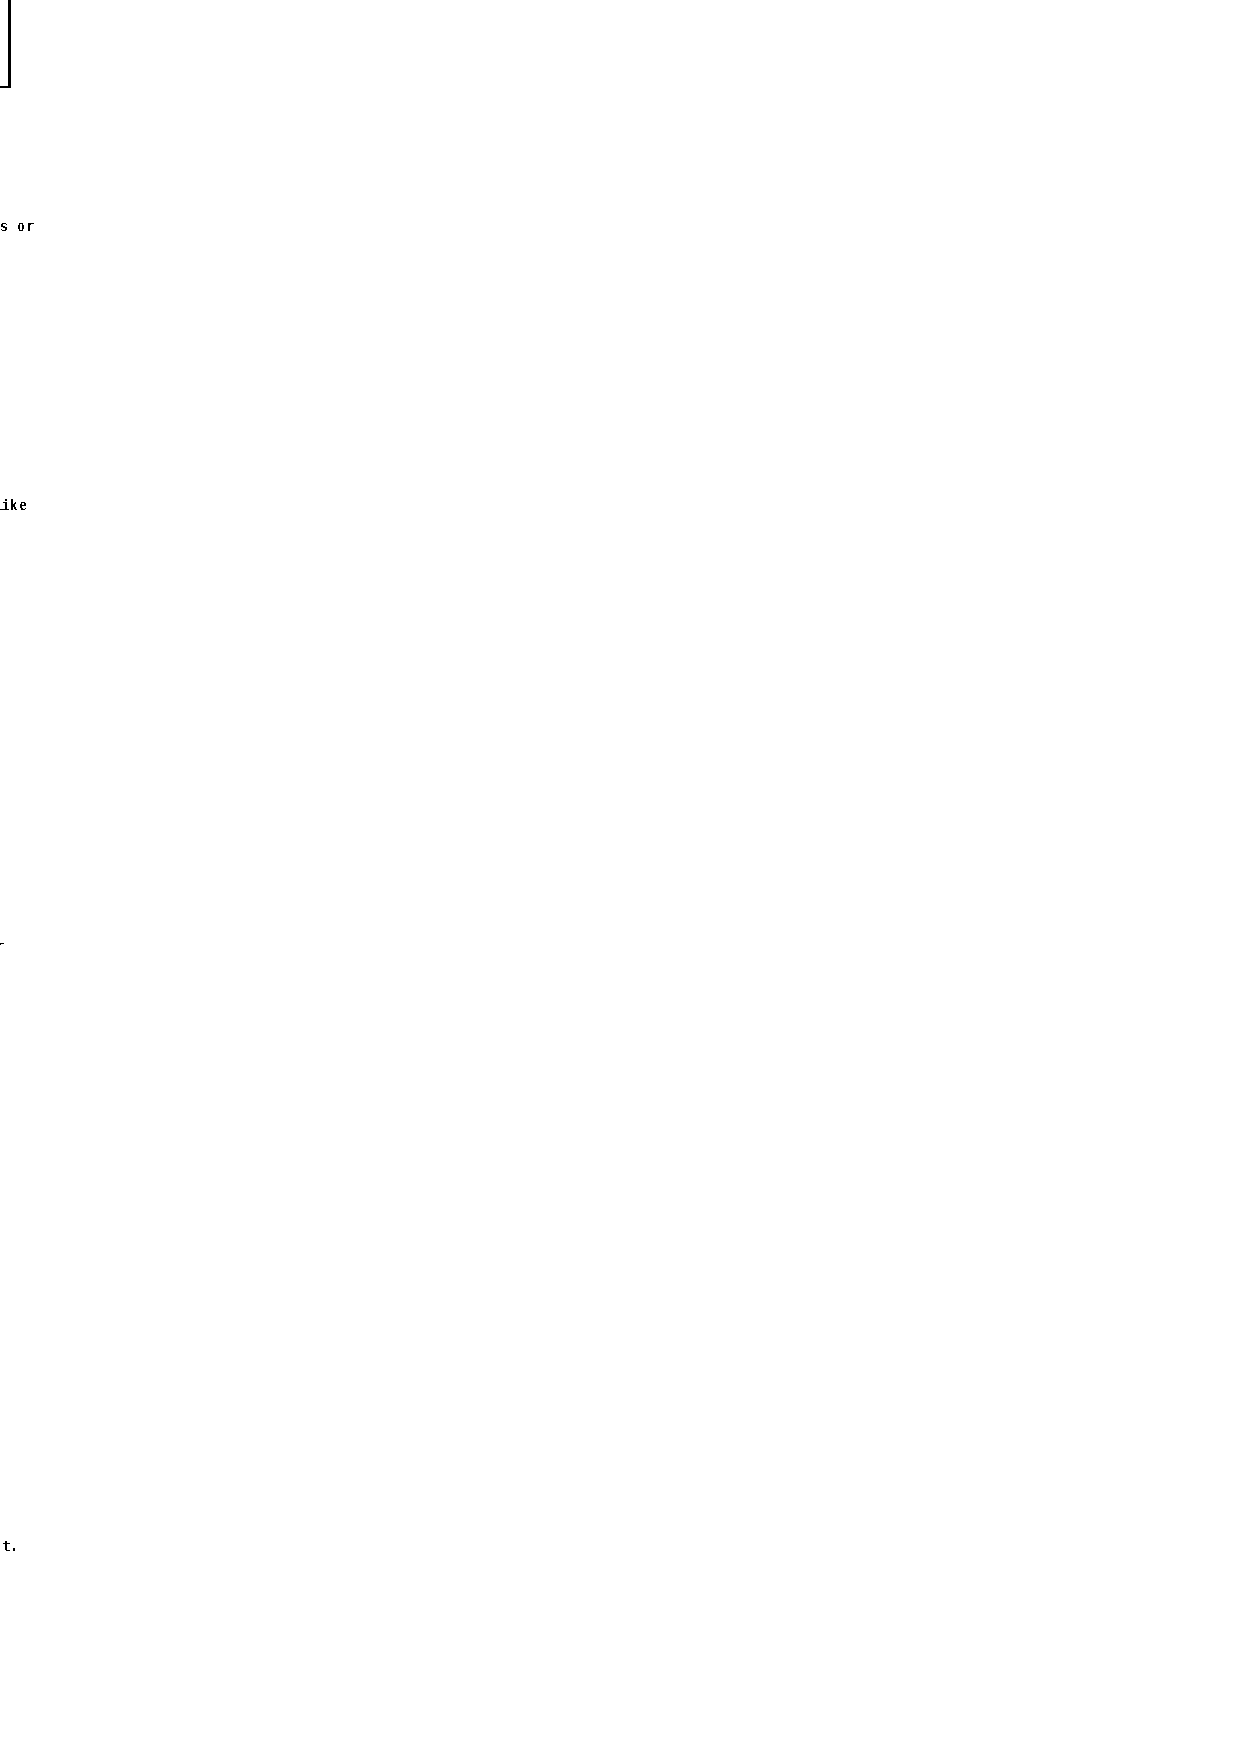
\includegraphics[trim=0 0 200 0, width=1.0\textwidth]{[VoiceChanger].pdf}}
  \end{center}
\end{figure}

\end{mdframed}
\vspace*{\baselineskip}

\end{document}
